\documentclass[12pt,letterpaper]{article}
\usepackage{graphicx,textcomp}
\usepackage{natbib}
\usepackage{setspace}
\usepackage{fullpage}
\usepackage{color}
\usepackage[reqno]{amsmath}
\usepackage{amsthm}
\usepackage{fancyvrb}
\usepackage{amssymb,enumerate}
\usepackage[all]{xy}
\usepackage{endnotes}
\usepackage{lscape}
\newtheorem{com}{Comment}
\usepackage{float}
\usepackage{hyperref}
\newtheorem{lem} {Lemma}
\newtheorem{prop}{Proposition}
\newtheorem{thm}{Theorem}
\newtheorem{defn}{Definition}
\newtheorem{cor}{Corollary}
\newtheorem{obs}{Observation}
\usepackage[compact]{titlesec}
\usepackage{dcolumn}
\usepackage{tikz}
\usetikzlibrary{arrows}
\usepackage{multirow}
\usepackage{xcolor}
\newcolumntype{.}{D{.}{.}{-1}}
\newcolumntype{d}[1]{D{.}{.}{#1}}
\definecolor{light-gray}{gray}{0.65}
\usepackage{url}
\usepackage{listings}
\usepackage{color}

\definecolor{codegreen}{rgb}{0,0.6,0}
\definecolor{codegray}{rgb}{0.5,0.5,0.5}
\definecolor{codepurple}{rgb}{0.58,0,0.82}
\definecolor{backcolour}{rgb}{0.95,0.95,0.92}

\lstdefinestyle{mystyle}{
	backgroundcolor=\color{backcolour},   
	commentstyle=\color{codegreen},
	keywordstyle=\color{magenta},
	numberstyle=\tiny\color{codegray},
	stringstyle=\color{codepurple},
	basicstyle=\footnotesize,
	breakatwhitespace=false,         
	breaklines=true,                 
	captionpos=b,                    
	keepspaces=true,                 
	numbers=left,                    
	numbersep=5pt,                  
	showspaces=false,                
	showstringspaces=false,
	showtabs=false,                  
	tabsize=2
}
\lstset{style=mystyle}
\newcommand{\Sref}[1]{Section~\ref{#1}}
\newtheorem{hyp}{Hypothesis}

\title{Problem Set 1}
\date{Due: October 1, 2023}
\author{Applied Stats/Quant Methods 1\\Stefan Keel}

\begin{document}
	\maketitle
	
	\section*{Instructions}
	\begin{itemize}
	\item Please show your work! You may lose points by simply writing in the answer. If the problem requires you to execute commands in \texttt{R}, please include the code you used to get your answers. Please also include the \texttt{.R} file that contains your code. If you are not sure if work needs to be shown for a particular problem, please ask.
\item Your homework should be submitted electronically on GitHub.
\item This problem set is due before 23:59 on Sunday October 1, 2023. No late assignments will be accepted.
\item Total available points for this homework is 80.
	\end{itemize}
	
	\vspace{1cm}
	\section*{Question 1 (40 points): Education}

A school counselor was curious about the average of IQ of the students in her school and took a random sample of 25 students' IQ scores. The following is the data set:\\

\lstinputlisting[language=R, firstline=40, lastline=40]{PS01_keels_answers.R}  

\textbf{Solution 0.1}: The average IQ of the students in her school is 98.44. This was calculated with following line of code in R:
\begin{verbatim}
	mean(y)
	\end{verbatim}

\begin{enumerate}
	\item Find a 90\% confidence interval for the average student IQ in the school.\\
	
\textbf{Solution 1.1}: 90\% of the true mean of the schools student IQ falls between 93.95993 and 102.92007.\\
As N smaller than 30, I opted for a t.distribution and therefore the qt function to find the standard error and subsequently the confidence interval. In the R code I calculated the length, standard deviation and sum of error, and standard error by hand. The fast way to find the confidence interval can be found below. 

\begin{verbatim}
	st_error <- qt(0.950, df = length(y) - 1) * (sd(y) / sqrt(length(y)))
	CI_lower <- mean(y) - st_error
	CI_higher <- mean(y) + st_error
	print(c(CI_lower, mean(y), CI_higher))
	93.95993  98.44000 102.92007
\end{verbatim}

	
	\item Next, the school counselor was curious  whether  the average student IQ in her school is higher than the average IQ score (100) among all the schools in the country.\\ 
	
	\noindent Using the same sample, conduct the appropriate hypothesis test with $\alpha=0.05$.
	
	\textbf{Solution 1.2}: P-Value is 0.7215383 and therefore greater than $\alpha=0.05$. As the P-Value is bigger than 0.05 we accept the Null-Hypotheses.\\
	\\
	Assumptions:
	\begin{itemize}
		\item Conducted IQ test at school is accurate for students IQs
		\item Average IQ scores in country was/is 100
		\item Sample group is fair
	\end{itemize}
	
My hypothesis: whether school IQ is higher than 100. 
Therefore it is a one-sided test.
	
Stating the Hypothesis: The hypothesis states that the average IQ of school students is higher than the average country IQ.\\
H0 mu is smaller equal than  100 \\
HA mu is greater than 100
\\
Following code was used to calculate P-Value and t.test conducted for proof of P-Value:
\begin{verbatim}
t_stat <- (mean(y)-100)/(sd(y)/sqrt(length(y))) 
P_value <- pt(t_stat, df = length(y)-1, lower.tail = FALSE)
print(P_value)
P_Value = 0.7215383

t_test <- t.test(y, mu = 100, alternative = 'greater') 
print(t_test)
data:  yt = -0.59574, df = 24, p-value = 0.7215
alternative hypothesis: true mean is greater than 100
95 percent confidence interval:  93.95993      Inf
sample estimates: mean of x     98.44 
\end{verbatim}

\end{enumerate}

\newpage

	\section*{Question 2 (40 points): Political Economy}

\noindent Researchers are curious about what affects the amount of money communities spend on addressing homelessness. The following variables constitute our data set about social welfare expenditures in the USA. \\
\vspace{.5cm}


\begin{tabular}{r|l}
	\texttt{State} &\emph{50 states in US} \\
	\texttt{Y} & \emph{per capita expenditure on shelters/housing assistance in state}\\
	\texttt{X1} &\emph{per capita personal income in state} \\
	\texttt{X2} &  \emph{Number of residents per 100,000 that are "financially insecure" in state}\\
	\texttt{X3} &  \emph{Number of people per thousand residing in urban areas in state} \\
	\texttt{Region} &  \emph{1=Northeast, 2= North Central, 3= South, 4=West} \\
\end{tabular}

\vspace{.5cm}
\noindent Explore the \texttt{expenditure} data set and import data into \texttt{R}.
\vspace{.5cm}
\vspace{.5cm}
\begin{itemize}

\item
Please plot the relationships among \emph{Y}, \emph{X1}, \emph{X2}, and \emph{X3}? What are the correlations among them (you just need to describe the graph and the relationships among them)?
\vspace{.5cm}

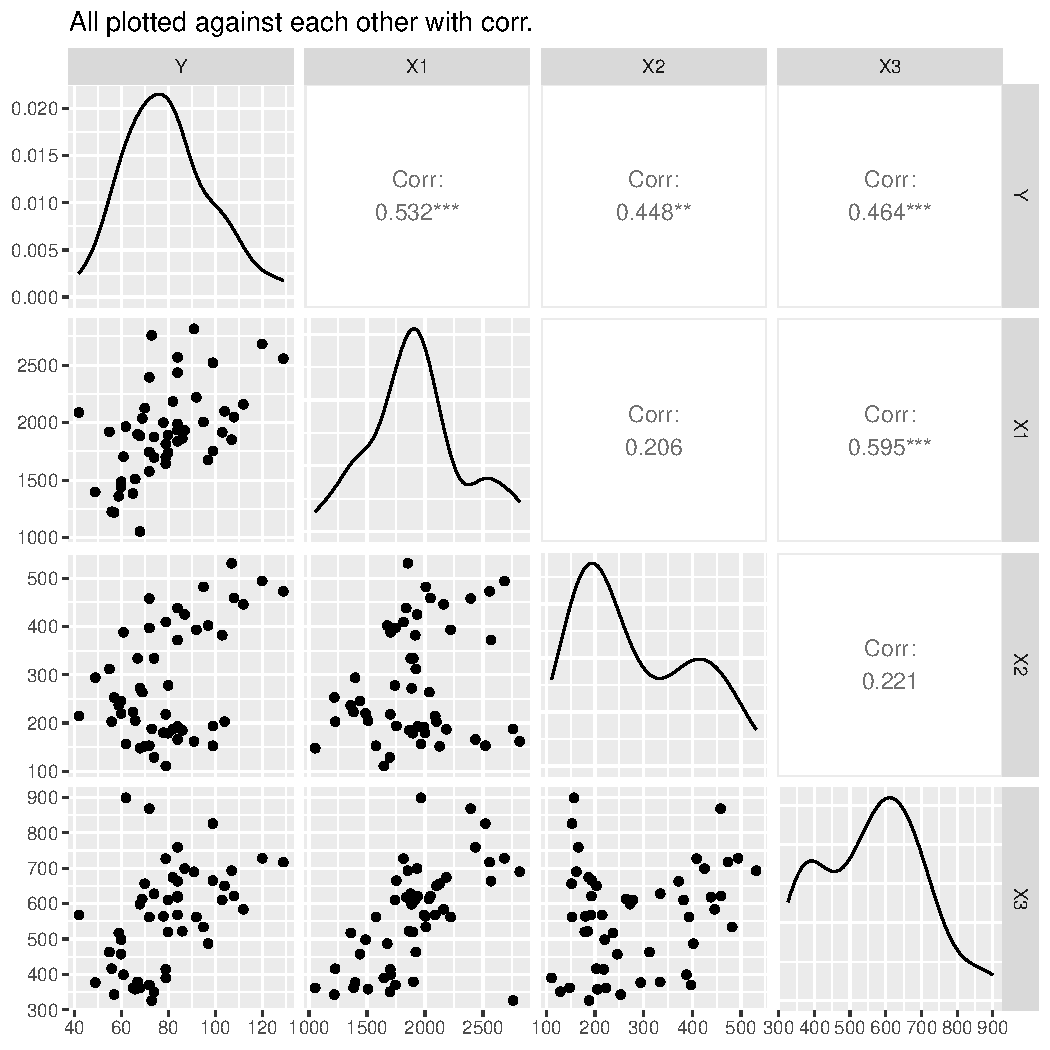
\includegraphics[width=.50\textwidth]{plot2.pdf} \\

\textbf{Solution 2.1}: From visual interpretation: 
\item Strongest correlation X1 and X3 with some outliers
\item Y and X1 also seem to have a good correlation but more outliers
\item Y and X2 as well as X3 seem to have medium correlation
\item X2 in combination with X2 and X3 seems to have very little correlation
This visual interpretation is backed by the correlation numbers the plot calculated. \\

It would also be possible to plot each combination seperately but it was too tiresome. Therefore I searched the internet (URL in R file) for a code/package that combined it in one plot.\\
Exmpaple of single plotting:\\
\includegraphics[width=.50\textwidth]{plot1.pdf} \\

The code for the 4 by 4 plot with corr.:
\begin{verbatim}
	pdf("plot2.pdf")ggpairs(expenditure[,2:5]) +  
	ggtitle("All plotted against each other with corr.")
	dev.off()
\end{verbatim}

\item
Please plot the relationship between \emph{Y} and \emph{Region}? On average, which region has the highest per capita expenditure on housing assistance?
\vspace{.5cm}

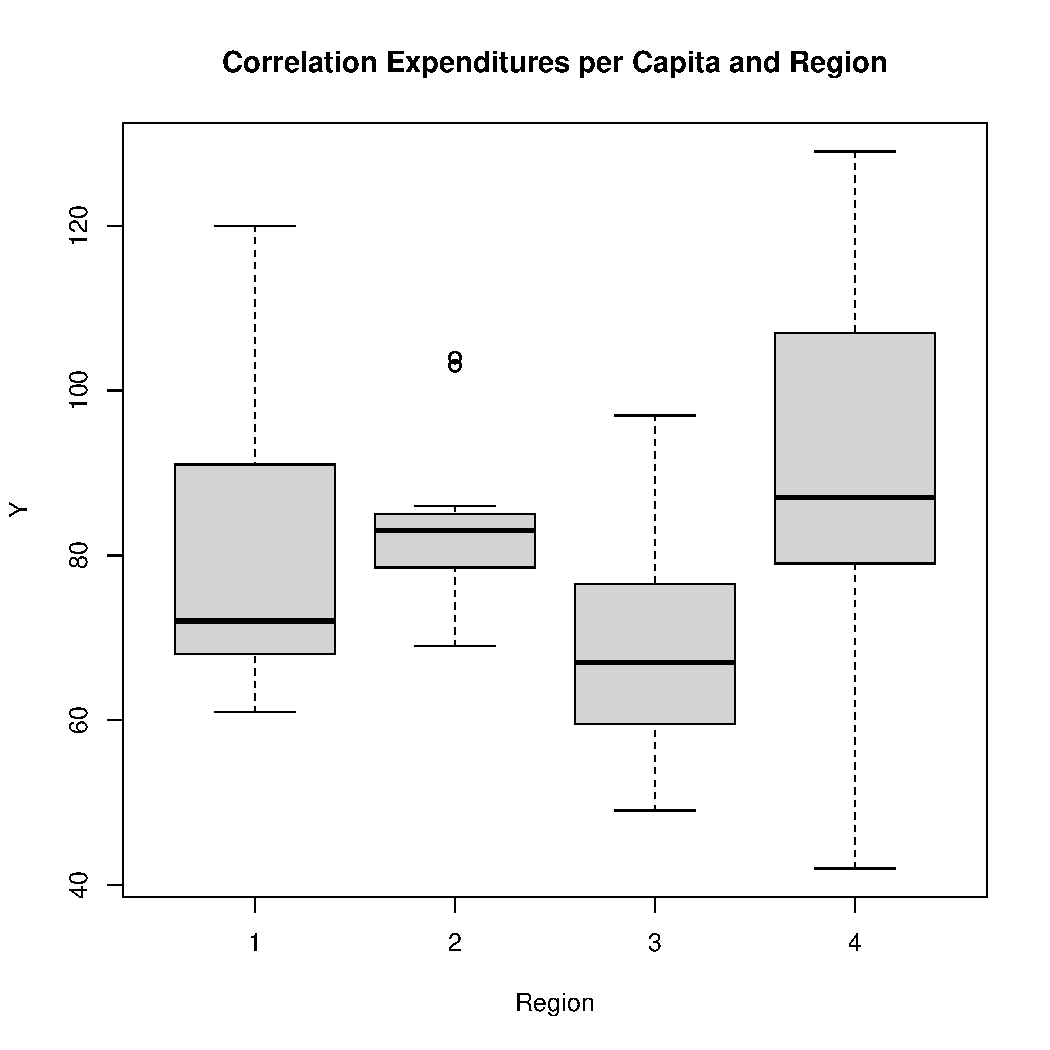
\includegraphics[width=.50\textwidth]{plot3.pdf} \\

\textbf{Solution 2.2}: Looking at the boxplot that also indicates the mean, we can see that Region 4 has the highest per capita expenditure on housing assistance. After calculating the means of each Region it can be stated that \textbf{on average Region 4 has with 88.30769 the highest per capita expenditure on housing assistance.}
\\
Used code in R:
\begin{verbatim}
pdf("plot3.pdf")boxplot(Y~Region,data = expenditure, 
main ="Correlation Expenditures per Capita and Region")
dev.off()
	
for(i in 1:4) 
{   
nam <- paste("Region", i, sep = "")  assign(nam, 
expenditure[expenditure$Region == i,])
}
mean(Region1$Y)
[1] 79.44444 
mean(Region2$Y)
[1] 83.91667
mean(Region3$Y)
[1] 69.1875
mean(Region4$Y)
[1] 88.30769
\end{verbatim}

\item
Please plot the relationship between \emph{Y} and \emph{X1}? Describe this graph and the relationship. Reproduce the above graph including one more variable \emph{Region} and display different regions with different types of symbols and colors.
\end{itemize}

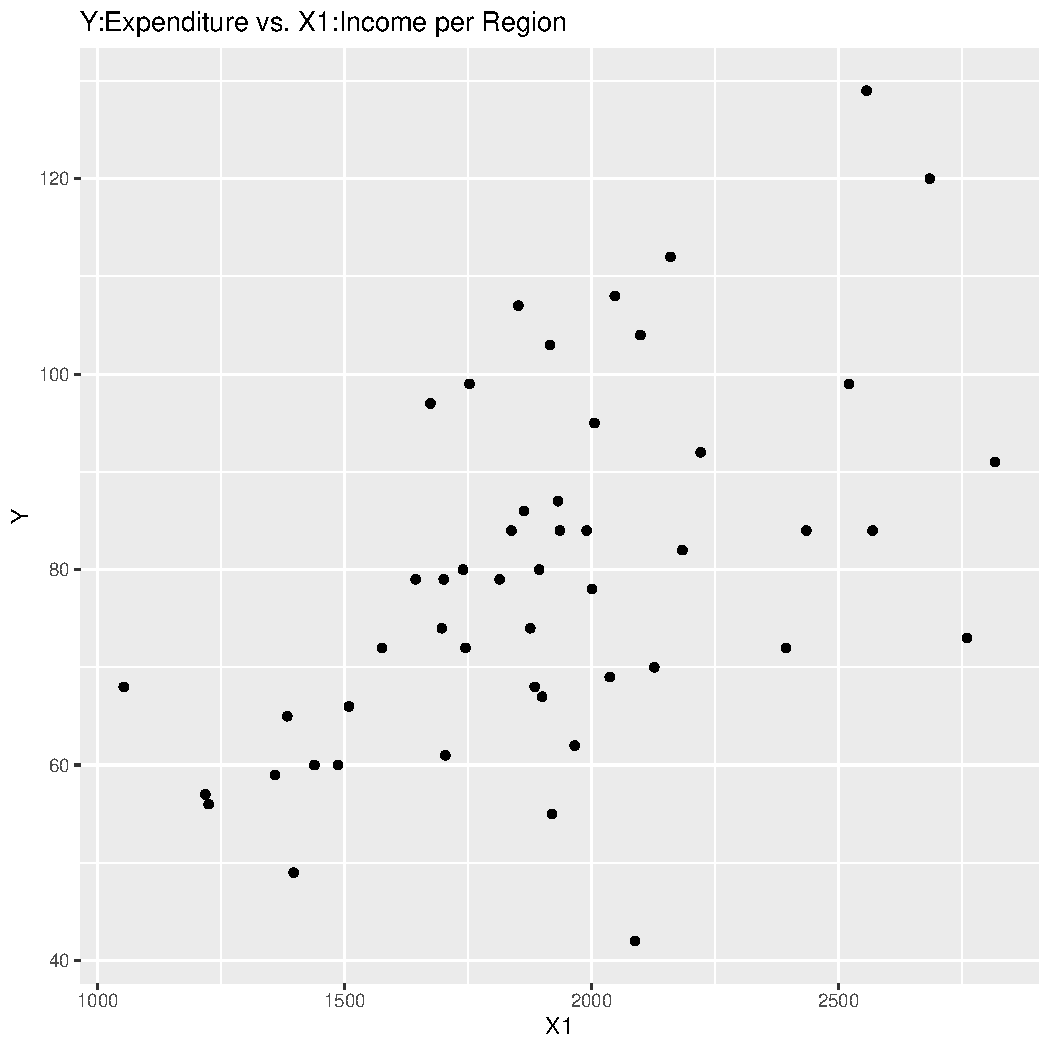
\includegraphics[width=.50\textwidth]{plot4.pdf} \\
\textbf{Solution 2.3.1}: Visual interpretatione. As mentioned before Y and X1 have a moderate positive correlation with some outliers. Most values lie between Y: 60 to 90 and X1: 1500 - 2000.\\

This code was used to visualise the correltaion Y and X1:
\begin{verbatim}
pdf("plot4.pdf")
ggplot(data = expenditure) +  
geom_point(mapping = aes(y = Y, x = X1)) +  
ggtitle("Y:Expenditure vs. X1:Income per Region")
dev.off()
\end{verbatim}

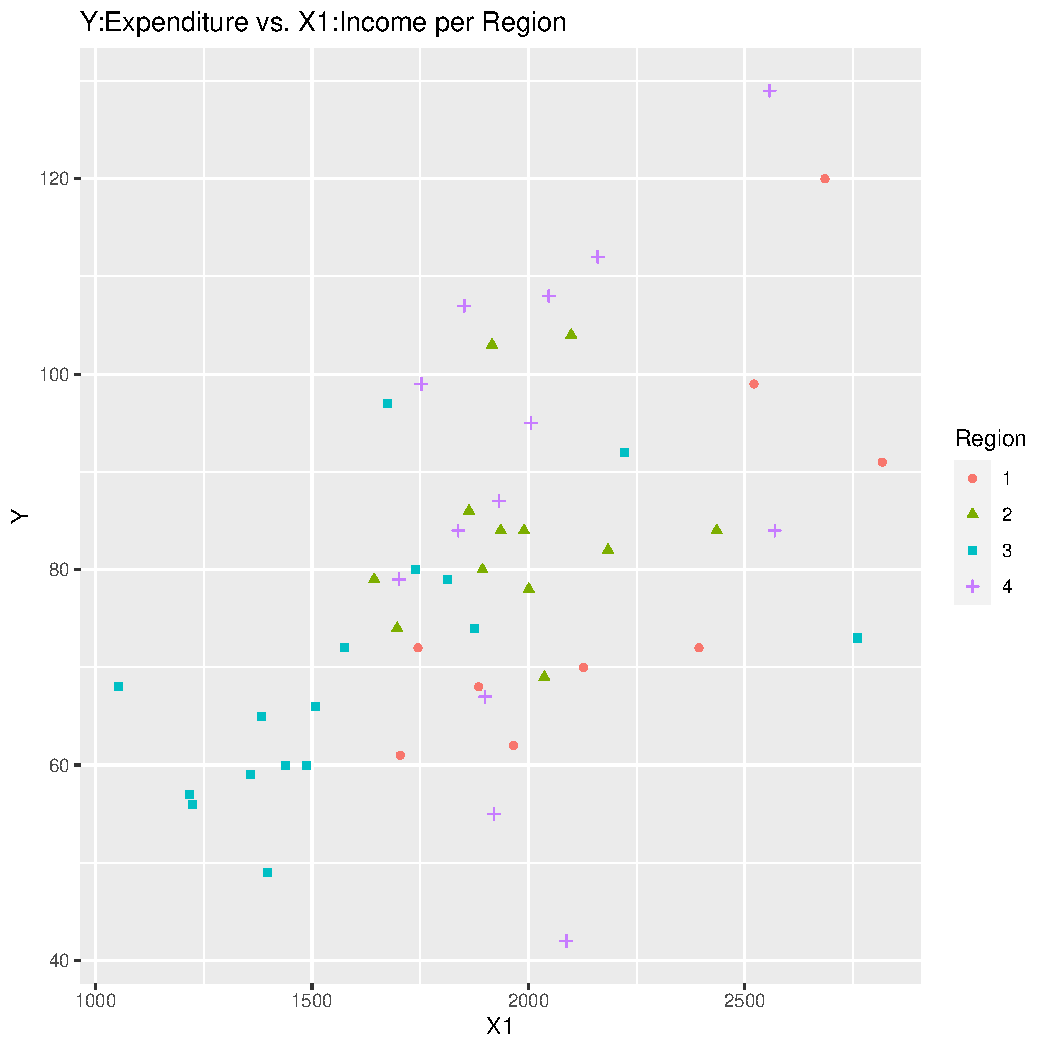
\includegraphics[width=.85\textwidth]{plot5.pdf} \\

\textbf{Solution 2.3.2}
\begin{itemize}
	\item Region 1 (Mean Expenditure: 79.44) is spread the furthest although most of the points are with low income and low expenditure.
	\item Region 2 (Mean Expenditure: 83.91) could be described as the best balanced between income and expenditure
	\item Region 3 (Mean Expenditure: 69.18) is spread the widest but most values are concentrated in the lower left corner.
	\item Region 4 (Mean Expenditure: 88.30) has the highest expenditure. This can be seen on the graph as most income is centered between 1700 and 2200. In comparison with other regions, region 4 has a big spread in the expenditures compared to other regions with similar income (which are not as far spread)
\end{itemize}

This code was used to enhance the previous code with colours and shapes for a better distinction.
\begin{verbatim}
	pdf("plot5.pdf")
	ggplot(data = expenditure) +    
	geom_point(mapping = aes(y = Y, x = X1, colour = as.factor(Region), 
	shape = as.factor(Region))) + 
	labs(colour="Region", shape = "Region") +  
	ggtitle("Y:Expenditure vs. X1:Income per Region")
	dev.off()
\end{verbatim}


\end{document}
